% =====================================================================
% Pretrained tabular transformers as low-N surrogates for vocal-fold models
% Draft skeleton. Portable article class (switch to REVTeX/JASA later).
% Compile: pdflatex main && bibtex main && pdflatex main && pdflatex main
% Figures live in sibling result folders; see \graphicspath below.
% =====================================================================
\documentclass[11pt]{article}

\usepackage[margin=1in]{geometry}
\usepackage{graphicx}
\usepackage{booktabs}
\usepackage{amsmath,amssymb}
\usepackage{xcolor}
\usepackage{subcaption}
\usepackage[numbers,sort&compress]{natbib}
\usepackage[hidelinks]{hyperref}

\graphicspath{{../Beam_Membrane/figs/}{../TBCM/figs/}{../JASA/figs/}}

% Provisional / TODO markers (toggle \draftmode to hide)
\newif\ifdraftmode \draftmodetrue
\newcommand{\todo}[1]{\ifdraftmode{\color{red}\textbf{[TODO: #1]}}\fi}
\newcommand{\prov}[1]{{\color{orange}#1}} % provisional (e.g. ACFL)

% Lightweight siunitx fallbacks (portable; swap for \usepackage{siunitx} later)
\providecommand{\second}{s}
\newcommand{\num}[1]{#1}
\newcommand{\SI}[2]{#1\,#2}

\title{Pretrained tabular transformers as low-$N$ surrogates for
vocal-fold models: a no-source alternative to transfer learning}

\author{Benjamin Gladney \and Callum Camazzola \and Sean D. Peterson \and
Jes\'us Parra \and Emiro Ibarra \and Mat\'ias Za\~nartu}
\date{\today}

\begin{document}
\maketitle

\begin{abstract}
Physically based vocal-fold models predict phonatory outputs from muscle
activations and subglottal pressure but are expensive to evaluate. Machine-
learning \emph{surrogates} can replace them for the forward problem, yet their
accuracy collapses when only a handful of simulations are available---the
low-sample regime that matters in practice. We ask whether a pretrained tabular
foundation model, TabPFN, is an effective low-$N$ surrogate for these models,
taking purpose-built transfer learning from a cheap source model as the strong
baseline it must beat. Across vocal-fold models of increasing structural
distance from the source---most importantly the finite-element Beam--Membrane
(BM) model---TabPFN matches or beats the transfer baseline at every training
size, with the largest margins at low $N$, on both accuracy ($R^2$) and error
(normalized RMSE), while requiring no source model and no training. Performance
is governed by source--target alignment: on the far, finite-element domain the
cheap source is a poor prior and TabPFN wins outright. It reconstructs the full
$(a_{CT}\times a_{TA})$ activation map from as few as $N{=}10$ samples and
extends naturally from $F_0$/SPL to physiological outputs (collision pressure,
AC flow, CPP) through a single multi-output head.
\end{abstract}

% =====================================================================
\section{Introduction}
\label{sec:intro}
Physically based models of the vocal folds---lumped body-cover models and
higher-fidelity continuum (finite-element) models---predict phonatory outputs
from muscle activations and subglottal pressure, but are costly to evaluate at
scale. Prior work showed that machine-learning surrogates can replace these
simulations for the \emph{forward} problem, yet their accuracy degrades sharply
when few training simulations are available. That degradation motivated
\emph{transfer learning}: train a surrogate on a cheap source model (the
body-cover model, BCM) and adapt it to an expensive target with a small number
of target simulations \citep{TODOprior}.

Transfer learning, however, requires a trained source model plus target
adaptation, and only pays off when the source and target are aligned. This
paper asks a complementary question:
\begin{quote}
\emph{Can a pretrained tabular foundation model act as a low-$N$ surrogate for
vocal-fold models, competing with---or replacing---transfer-learning
strategies?}
\end{quote}
We study TabPFN \citep{hollmann2025tabpfn}, a transformer pretrained once on
millions of synthetic tabular problems and then frozen: it fits a new task
in-context in a single forward pass, with no per-task training and no source
model. Casting both methods as ``pretrained''---TabPFN on a synthetic prior,
transfer on the BCM source---puts them on equal footing and isolates the
variable that decides the contest: source--target alignment.

% =====================================================================
\section{Methods}
\label{sec:methods}

\subsection{Physical vocal-fold models and data}
\label{sec:models}
All models share inputs (muscle activations $a_{CT}$, $a_{TA}$, lateral
cricoarytenoid $a_{LCA}$, and subglottal pressure $P_s$) and the base outputs
$F_0$ and SPL; the richer outputs (Sec.~\ref{sec:richer}) are added for the
target.
\begin{itemize}
  \item \textbf{Beam--Membrane (BM)} --- \emph{main case.} A finite-element /
  continuum model; the expensive, structurally distinct target. It is the
  \emph{far} domain relative to the BCM source, where the low-$N$ question is
  sharpest. \num{4647} phonating samples (filtered $\mathrm{ACFL}>30$).
  \item \textbf{Triangular Body-Cover Model (TBCM)} --- \emph{secondary case.}
  Lumped-element, same family as BCM; sampled on a $40\times40$
  $(a_{CT}\times a_{TA})$ grid, providing real ODE ground-truth activation maps
  (Sec.~\ref{sec:maps}).
  \item \textbf{Body-Cover Model (BCM)} --- the cheap \emph{source} model
  (\num{360000} samples) for all transfer learning.
\end{itemize}
\todo{add model equations / refs; cite Parra TBCM and BM solver}

\subsection{Low-$N$ regression strategies}
\label{sec:strategies}
\paragraph{TabPFN (no source).} A pretrained tabular transformer applied with
per-output standardization. We evaluate single-output heads and a stacked
\emph{multi-output} head (Sec.~\ref{sec:richer}). No training is performed
beyond the in-context fit.

\paragraph{TransRF (transfer).} A BCM-source random forest combined with
residual-correction and feature-augmentation sub-models, fused by non-negative
ensemble weights. The source RF is trained once (per-domain pretraining); only
the sub-models and weights are fit per task.

\paragraph{Evaluation.} For each training size $N\in\{10,20,50,100,200,500\}$,
models train on $N$ target rows and are evaluated on a disjoint held-out pool of
up to \num{1000} rows; we report mean $\pm$ s.d.\ over 5 seeds. We use $R^2$ and
the range-normalized RMSE,
\begin{equation}
  \mathrm{nRMSE} = \frac{\sqrt{\tfrac{1}{n}\sum_i (y_i-\hat y_i)^2}}
                        {\max_i y_i - \min_i y_i},
\end{equation}
rather than MAPE, because SPL is negative and collision pressure / CPP cross
zero, making MAPE ill-defined.

% =====================================================================
\section{Results}
\label{sec:results}

\subsection{Result 1 --- Accuracy and error versus training size}
\label{sec:metrics}
On the far (BM) domain, TabPFN beats transfer at every $N$ and on both metrics,
with the largest margins in the low-$N$ regime (Fig.~\ref{fig:metrics},
Table~\ref{tab:metrics}). The cheap BCM source is a poor prior for the
finite-element BM model, so transfer cannot lean on it and TabPFN---which needs
no source---wins outright.

\begin{figure}[t]
  \centering
  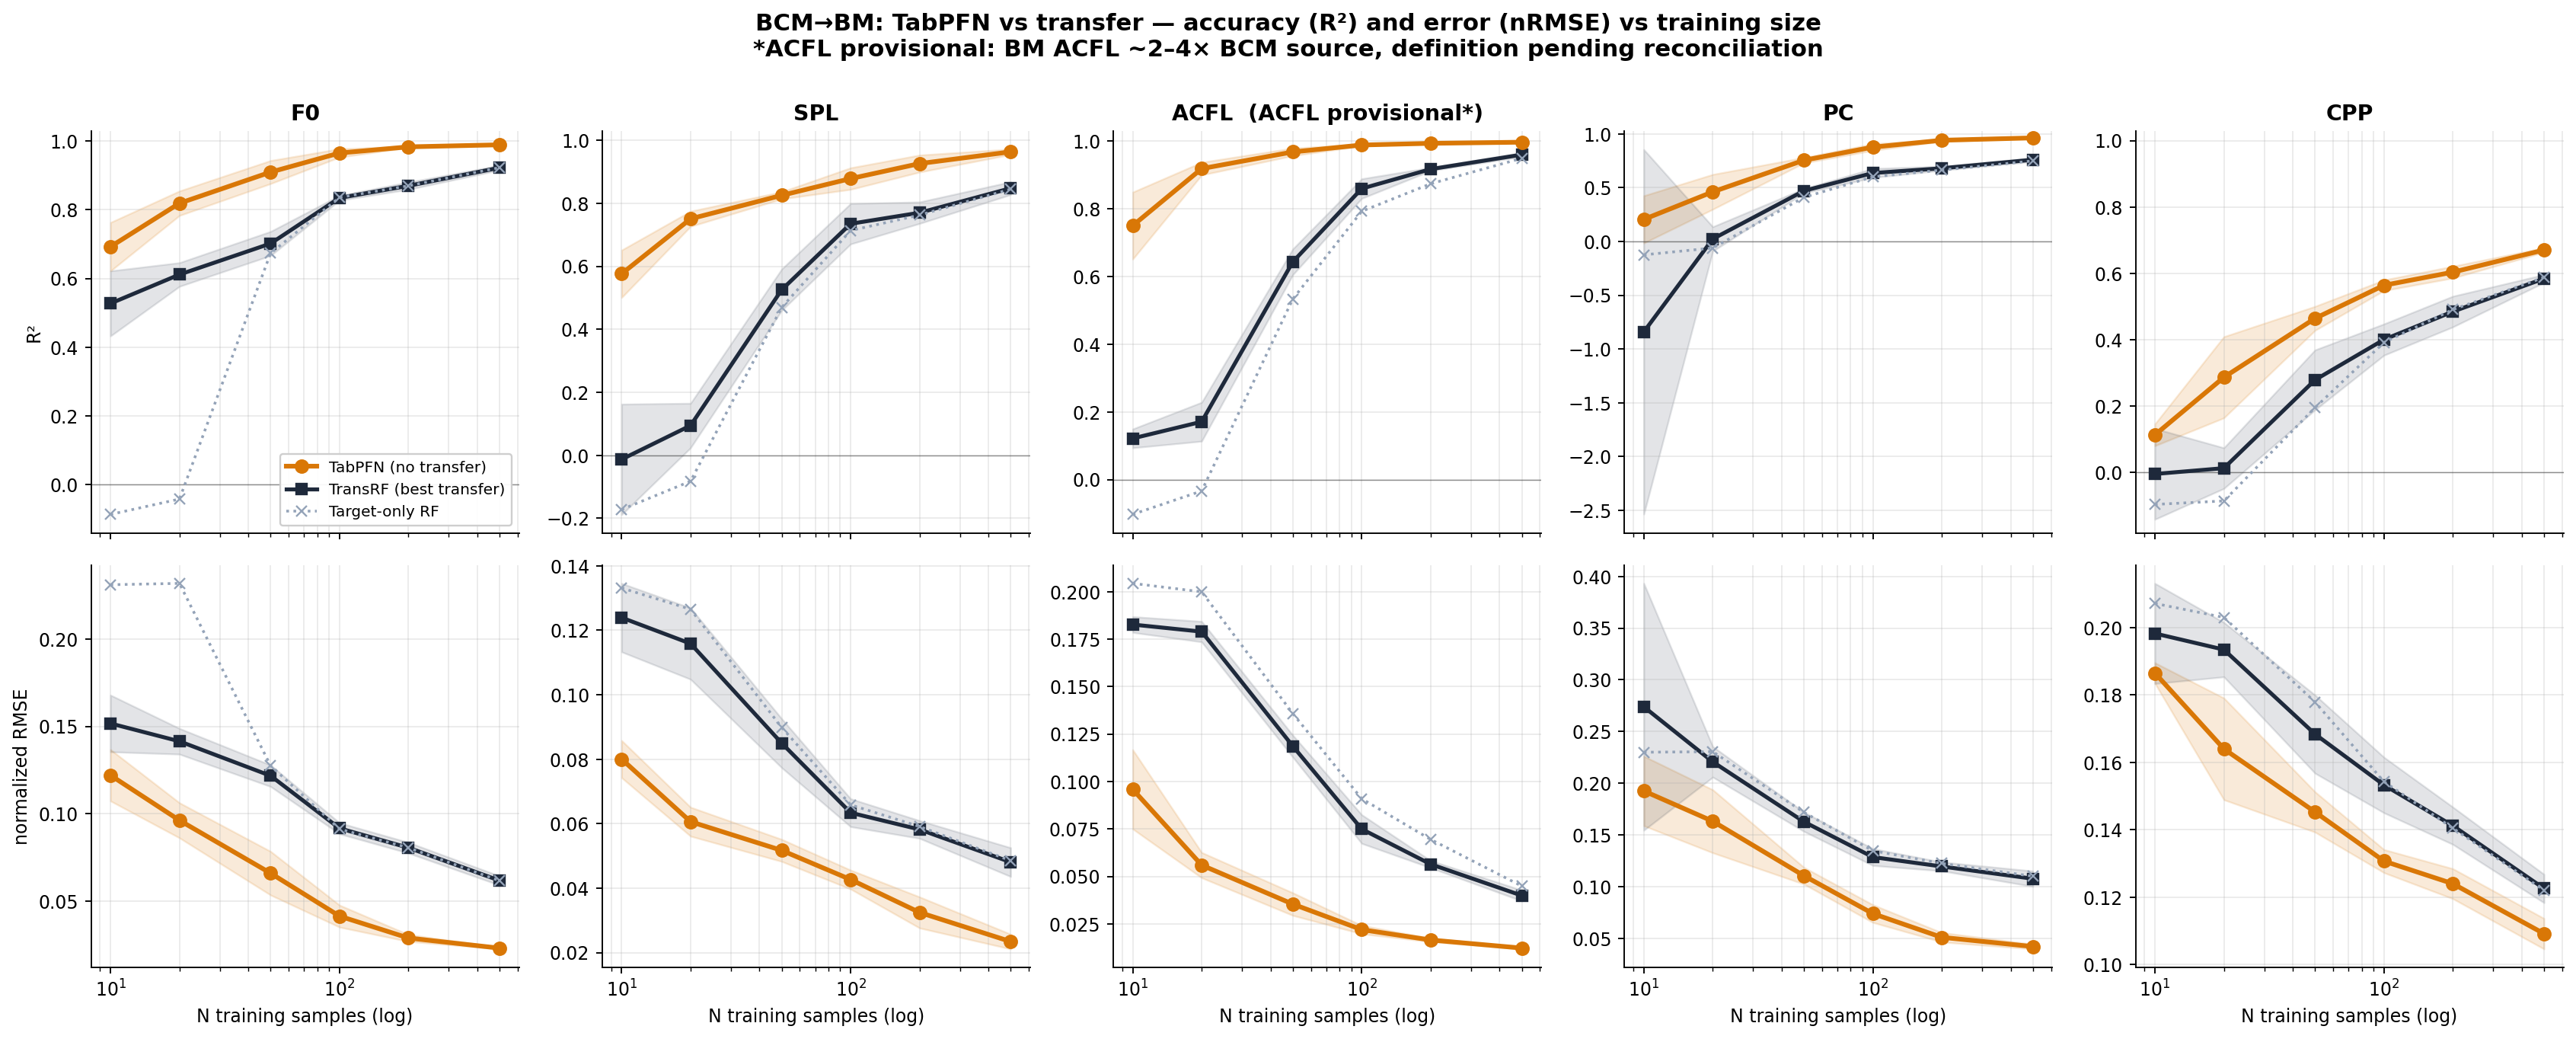
\includegraphics[width=\linewidth]{bm_ext_metrics_vs_n.png}
  \caption{BCM$\to$BM: $R^2$ (top) and normalized RMSE (bottom) versus training
  size $N$ for each output, TabPFN vs.\ TransRF vs.\ a target-only baseline
  (mean $\pm$ s.d., 5 seeds). \prov{ACFL provisional; see Sec.~\ref{sec:richer}.}}
  \label{fig:metrics}
\end{figure}

\begin{table}[t]
  \centering
  \caption{$R^2$ on BM (TabPFN single / TransRF) at $N{=}50$ and $N{=}200$.}
  \label{tab:metrics}
  \begin{tabular}{lcc}
    \toprule
    Output & $R^2$ @ $N{=}50$ & $R^2$ @ $N{=}200$ \\
    \midrule
    $F_0$         & 0.91 / 0.70 & 0.98 / 0.87 \\
    SPL           & 0.82 / 0.53 & 0.93 / 0.77 \\
    \prov{ACFL}   & 0.97 / 0.64 & 0.99 / 0.92 \\
    PC            & 0.76 / 0.47 & 0.94 / 0.68 \\
    CPP           & 0.46 / 0.28 & 0.60 / 0.49 \\
    \bottomrule
  \end{tabular}
\end{table}

\subsection{Result 2 --- Activation-map reconstruction}
\label{sec:maps}
Beyond point accuracy, a useful surrogate must reconstruct the physiological
\emph{structure} of the $(a_{CT}\times a_{TA})$ control space. On TBCM (the
gridded model with real ODE ground truth), TabPFN reconstructs the full
motor-control map from as few as $N{=}10$ samples and converges toward the
ground truth as $N\to1000$ (Fig.~\ref{fig:maps}), with lower image-level error
than transfer at almost every $N$ (Table~\ref{tab:maperr}).

\begin{figure}[t]
  \centering
  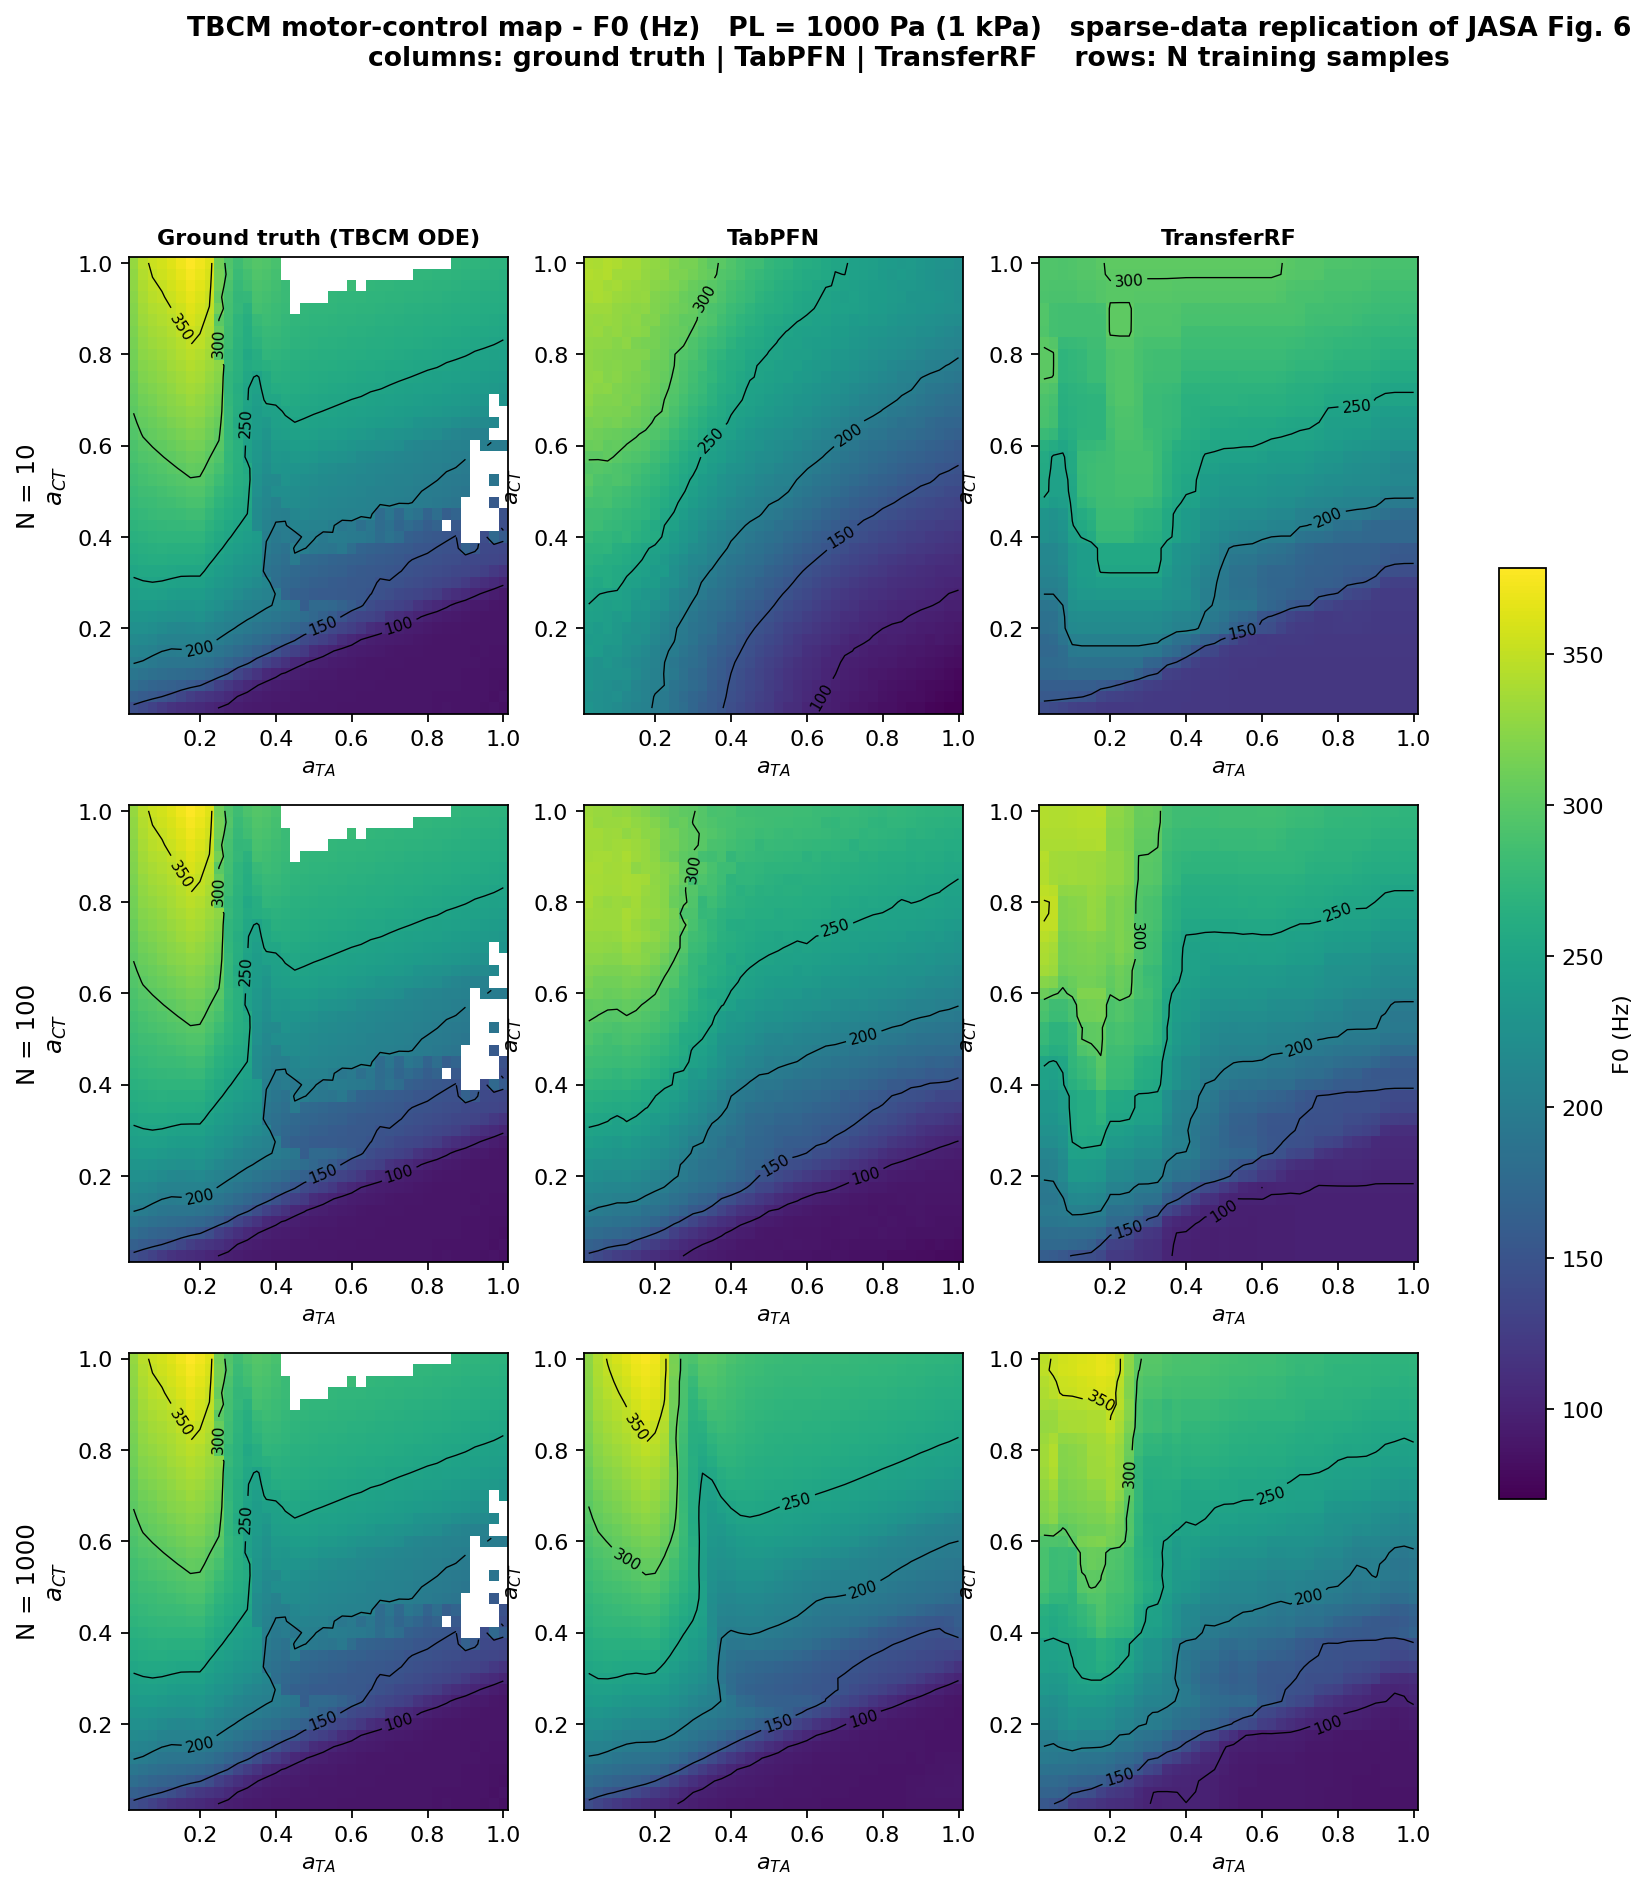
\includegraphics[width=\linewidth]{tbcm_motor_map_F0.png}
  \caption{TBCM $F_0$ motor-control maps. Rows: $N=10/100/1000$; columns: ODE
  ground truth, TabPFN, TransRF. SPL and signed-error maps in the supplement.}
  \label{fig:maps}
\end{figure}

\begin{table}[t]
  \centering
  \caption{Image-level error over all grid cells (MAE / RMSE), TabPFN vs.\
  TransRF. Lower is better.}
  \label{tab:maperr}
  \begin{tabular}{llcc}
    \toprule
    Output & $N$ & TabPFN (MAE/RMSE) & TransRF (MAE/RMSE) \\
    \midrule
    $F_0$ (Hz) & 10   & 20.3 / 25.3 & 23.0 / 26.6 \\
               & 100  & 6.3 / 9.8   & 8.6 / 11.6 \\
               & 1000 & 1.7 / 3.2   & 4.6 / 6.6 \\
    SPL (dB)   & 10   & 7.8 / 9.4   & 6.8 / 8.4 \\
               & 100  & 1.9 / 2.8   & 2.9 / 4.6 \\
               & 1000 & 0.6 / 1.4   & 1.8 / 3.0 \\
    \bottomrule
  \end{tabular}
\end{table}

\subsection{Result 3 --- Runtime: adaptation versus inference}
\label{sec:runtime}
A surrogate must be practical, not only accurate. We separate the one-time
per-domain pretraining from the per-task adaptation and inference
(Fig.~\ref{fig:runtime}). TransRF pays a \SI{279}{\second} one-time source-RF
build, then \SI{5.0}{\second} adaptation and \SI{1.9}{\second} inference per
task; TabPFN needs \emph{no} per-domain pretraining and no source data.
\todo{add network-free local-TabPFN inference bar once license-gated weights are
cached; current cloud inference includes network round-trip.}

\begin{figure}[t]
  \centering
  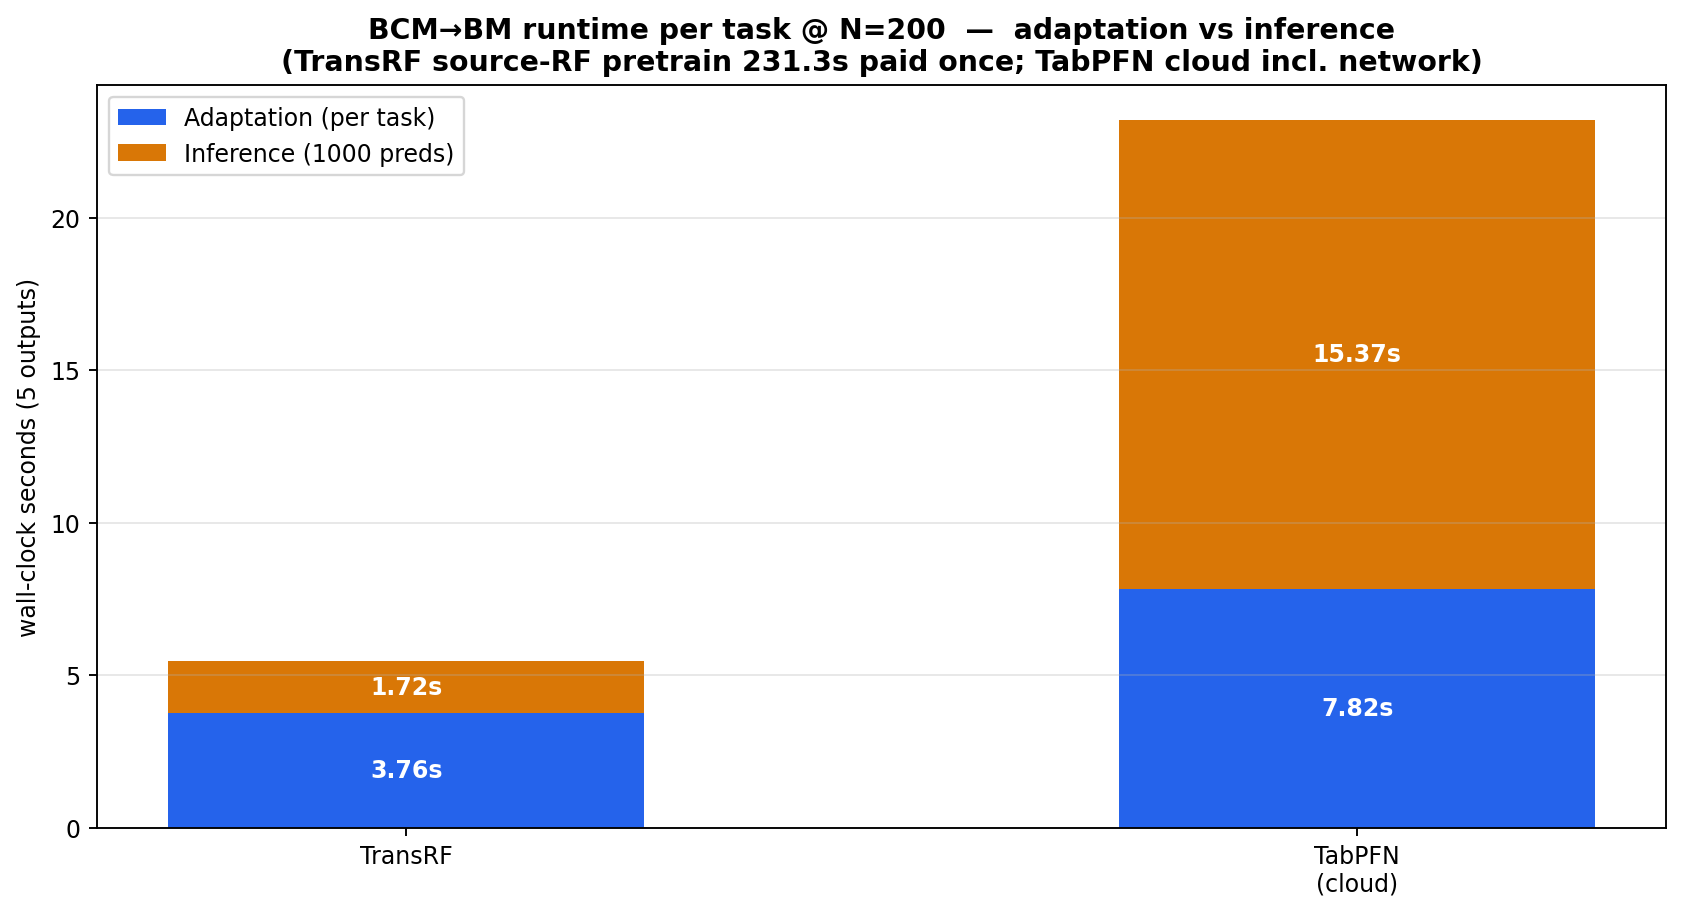
\includegraphics[width=0.8\linewidth]{bm_ext_runtime.png}
  \caption{Per-task runtime at $N{=}200$ (5 outputs): adaptation vs.\ inference.
  TransRF's source-RF pretraining (\SI{279}{\second}) is paid once. TabPFN cloud
  inference includes network round-trip.}
  \label{fig:runtime}
\end{figure}

\subsection{Result 4 --- Richer physiological outputs}
\label{sec:richer}
TabPFN extends from $F_0$/SPL to physiological outputs---collision pressure
(PC), AC flow (ACFL), and cepstral peak prominence (CPP)---at no extra
machinery. A single joint multi-output head predicts all outputs at once and
trails the dedicated single-output heads by only $\sim$0.05 $R^2$
(Fig.~\ref{fig:multihead}); we therefore lead with the multi-output setting and
report single heads as an ablation.
\prov{ACFL is provisional: BM AC flow currently runs $\sim$2--4$\times$ the BCM
source, a definition/scale nuance pending reconciliation with the source
routine; PC and CPP are scale-consistent.}

\begin{figure}[t]
  \centering
  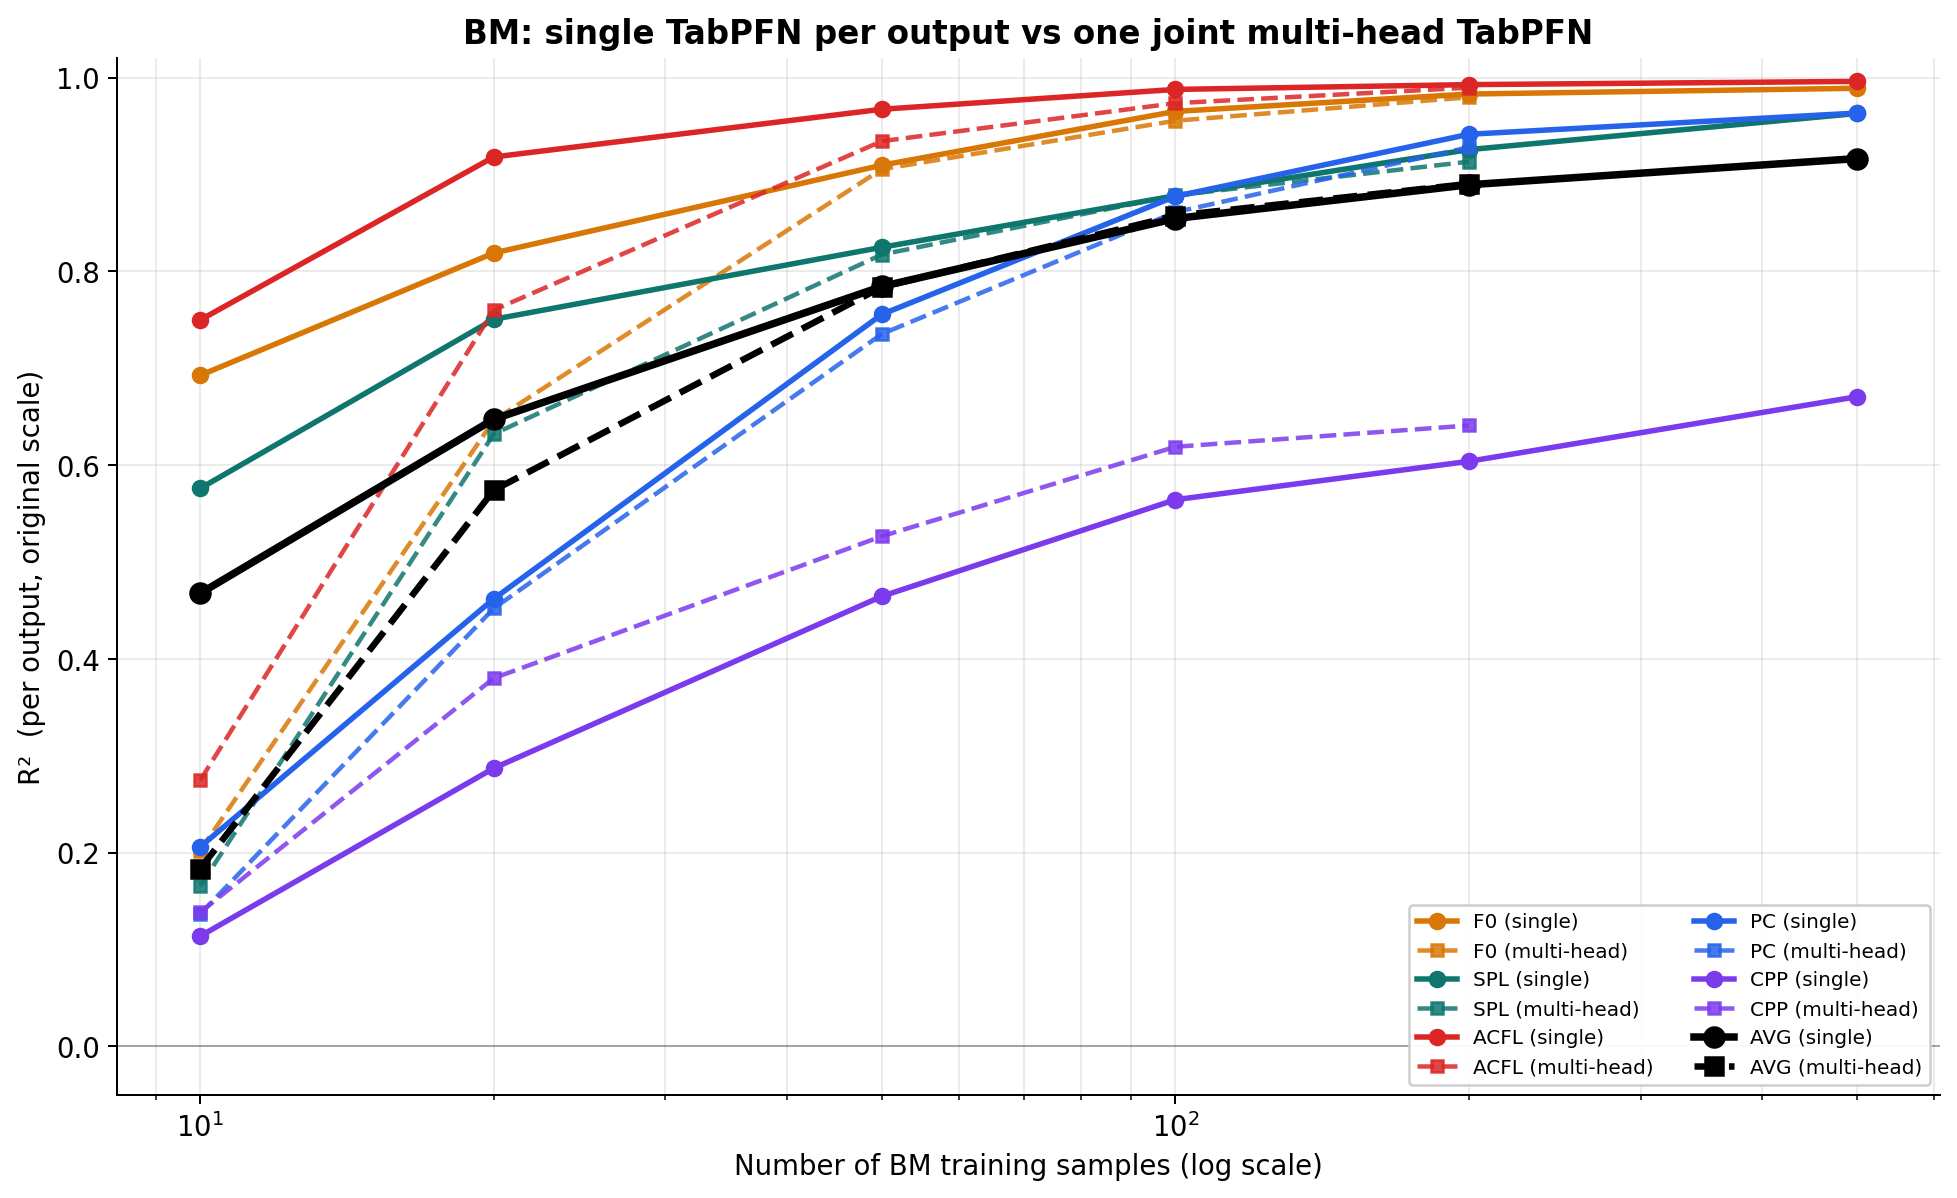
\includegraphics[width=0.85\linewidth]{bm_ext_multihead_vs_single.png}
  \caption{Single-output vs.\ joint multi-output TabPFN on BM ($R^2$ vs.\ $N$).
  The multi-head trails the singles marginally while delivering all outputs from
  one model; it is capped at $N{=}200$ by TabPFN's in-context size limit.}
  \label{fig:multihead}
\end{figure}

\subsection{Result 5 --- Structured missing modalities}
\label{sec:missing}
\todo{Reframe missing-data from random deletion to structured missing-modality:
drop a whole input/output modality (acoustic, aerodynamic, or physiological) in
$X\%$ of rows, mimicking an unavailable sensor; report accuracy vs.\ $X$ for
TabPFN vs.\ transfer. Figure to generate.}

% =====================================================================
\section{Discussion}
\label{sec:discussion}
The contest between a no-source pretrained surrogate and transfer learning is
governed by source--target alignment: on the far finite-element domain the BCM
prior is unhelpful and TabPFN dominates, whereas on closely aligned lumped
models transfer remains competitive. Because TabPFN needs no source model or
source data, it removes the per-domain pretraining and the dependence on a cheap
analogue altogether.

\paragraph{Toward the inverse problem (outlook).} The forward setting predicts
outputs from pressure and activations; the \emph{inverse} setting estimates
control or physiological variables from observable features (accelerometer,
acoustic, aerodynamic), where missing modalities arise naturally. TabPFN could
connect three prior lines---ML surrogate (forward), deterministic estimation of
$P_s$/collision pressure/activations, and probabilistic PBNN---but whether the
inverse problem belongs here or in a follow-up is left open. \todo{decide:
exploratory section vs.\ second paper.}

% =====================================================================
\section{Conclusion}
\label{sec:conclusion}
A pretrained tabular transformer is a practical, no-source, no-train low-$N$
surrogate for expensive vocal-fold models---competitive with, and on far domains
better than, purpose-built transfer learning, and extending naturally to
physiological outputs.

\bibliographystyle{plainnat}
\bibliography{refs}

\end{document}
